% Options for packages loaded elsewhere
\PassOptionsToPackage{unicode}{hyperref}
\PassOptionsToPackage{hyphens}{url}
%
\documentclass[
  ignorenonframetext,
  aspectratio=169]{beamer}
\title{Causal inference in analyzing administrative healthcare data:}
\subtitle{Can we integrate machine learning approaches within this
framework?}
\author{Ehsan Karim\\
\url{http://ehsank.com/}}
\date{Feb 23, 2021; CHSPR}

\usepackage{pgfpages}
\setbeamertemplate{caption}[numbered]
\setbeamertemplate{caption label separator}{: }
\setbeamercolor{caption name}{fg=normal text.fg}
\beamertemplatenavigationsymbolsempty
% Prevent slide breaks in the middle of a paragraph
\widowpenalties 1 10000
\raggedbottom
\setbeamertemplate{part page}{
  \centering
  \begin{beamercolorbox}[sep=16pt,center]{part title}
    \usebeamerfont{part title}\insertpart\par
  \end{beamercolorbox}
}
\setbeamertemplate{section page}{
  \centering
  \begin{beamercolorbox}[sep=12pt,center]{part title}
    \usebeamerfont{section title}\insertsection\par
  \end{beamercolorbox}
}
\setbeamertemplate{subsection page}{
  \centering
  \begin{beamercolorbox}[sep=8pt,center]{part title}
    \usebeamerfont{subsection title}\insertsubsection\par
  \end{beamercolorbox}
}
\AtBeginPart{
  \frame{\partpage}
}
\AtBeginSection{
  \ifbibliography
  \else
    \frame{\sectionpage}
  \fi
}
\AtBeginSubsection{
  \frame{\subsectionpage}
}
\usepackage{amsmath,amssymb}
\usepackage{lmodern}
\usepackage{iftex}
\ifPDFTeX
  \usepackage[T1]{fontenc}
  \usepackage[utf8]{inputenc}
  \usepackage{textcomp} % provide euro and other symbols
\else % if luatex or xetex
  \usepackage{unicode-math}
  \defaultfontfeatures{Scale=MatchLowercase}
  \defaultfontfeatures[\rmfamily]{Ligatures=TeX,Scale=1}
\fi
\usetheme[]{AnnArbor}
\usecolortheme{crane}
\usefonttheme{structurebold}
% Use upquote if available, for straight quotes in verbatim environments
\IfFileExists{upquote.sty}{\usepackage{upquote}}{}
\IfFileExists{microtype.sty}{% use microtype if available
  \usepackage[]{microtype}
  \UseMicrotypeSet[protrusion]{basicmath} % disable protrusion for tt fonts
}{}
\makeatletter
\@ifundefined{KOMAClassName}{% if non-KOMA class
  \IfFileExists{parskip.sty}{%
    \usepackage{parskip}
  }{% else
    \setlength{\parindent}{0pt}
    \setlength{\parskip}{6pt plus 2pt minus 1pt}}
}{% if KOMA class
  \KOMAoptions{parskip=half}}
\makeatother
\usepackage{xcolor}
\IfFileExists{xurl.sty}{\usepackage{xurl}}{} % add URL line breaks if available
\IfFileExists{bookmark.sty}{\usepackage{bookmark}}{\usepackage{hyperref}}
\hypersetup{
  pdftitle={Causal inference in analyzing administrative healthcare data:},
  hidelinks,
  pdfcreator={LaTeX via pandoc}}
\urlstyle{same} % disable monospaced font for URLs
\newif\ifbibliography
\usepackage{graphicx}
\makeatletter
\def\maxwidth{\ifdim\Gin@nat@width>\linewidth\linewidth\else\Gin@nat@width\fi}
\def\maxheight{\ifdim\Gin@nat@height>\textheight\textheight\else\Gin@nat@height\fi}
\makeatother
% Scale images if necessary, so that they will not overflow the page
% margins by default, and it is still possible to overwrite the defaults
% using explicit options in \includegraphics[width, height, ...]{}
\setkeys{Gin}{width=\maxwidth,height=\maxheight,keepaspectratio}
% Set default figure placement to htbp
\makeatletter
\def\fps@figure{htbp}
\makeatother
\setlength{\emergencystretch}{3em} % prevent overfull lines
\providecommand{\tightlist}{%
  \setlength{\itemsep}{0pt}\setlength{\parskip}{0pt}}
\setcounter{secnumdepth}{-\maxdimen} % remove section numbering
\newlength{\cslhangindent}
\setlength{\cslhangindent}{1.5em}
\newlength{\csllabelwidth}
\setlength{\csllabelwidth}{3em}
\newlength{\cslentryspacingunit} % times entry-spacing
\setlength{\cslentryspacingunit}{\parskip}
\newenvironment{CSLReferences}[2] % #1 hanging-ident, #2 entry spacing
 {% don't indent paragraphs
  \setlength{\parindent}{0pt}
  % turn on hanging indent if param 1 is 1
  \ifodd #1
  \let\oldpar\par
  \def\par{\hangindent=\cslhangindent\oldpar}
  \fi
  % set entry spacing
  \setlength{\parskip}{#2\cslentryspacingunit}
 }%
 {}
\usepackage{calc}
\newcommand{\CSLBlock}[1]{#1\hfill\break}
\newcommand{\CSLLeftMargin}[1]{\parbox[t]{\csllabelwidth}{#1}}
\newcommand{\CSLRightInline}[1]{\parbox[t]{\linewidth - \csllabelwidth}{#1}\break}
\newcommand{\CSLIndent}[1]{\hspace{\cslhangindent}#1}
\usepackage{graphicx,longtable,booktabs,amsmath,soul}
\usepackage{float}
\floatplacement{figure}{H}
\floatplacement{table}{H}
\usepackage{xcolor,lipsum,caption,natbib}
\def\bibfont{\small}
\ifLuaTeX
  \usepackage{selnolig}  % disable illegal ligatures
\fi

\begin{document}
\frame{\titlepage}

\begin{frame}{Outline}
\protect\hypertarget{outline}{}
\begin{enumerate}
\tightlist
\item
  Notations and Questions

  \begin{itemize}
  \tightlist
  \item
    Regression vs.~Propensity score (PS)
  \end{itemize}
\item
  Health care databases
\item
  High-dimensional propensity score (hdPS)

  \begin{itemize}
  \tightlist
  \item
    The original mechanism
  \item
    \textcolor{blue}{Machine learning-based hdPS}
  \item
    \textcolor{blue}{AI-based hdPS}
  \item
    \textcolor{blue}{Future directions}
  \end{itemize}
\item
  Examples in Canadian data
\end{enumerate}
\end{frame}

\begin{frame}{Reference Preview}
\protect\hypertarget{reference-preview}{}
Will be primarily discussing Schneeweiss (2018). Will also briefly
mention Karim, Pang, and Platt (2018),Weberpals et al. (2021), Zivich
and Breskin (2021).

\begin{itemize}
\tightlist
\item
  Schneeweiss (2018) Clinical Epidemiology
\item
  Karim et al.~(2018) Epidemiology
\item
  Weberpals et al.~(2021) Epidemiology
\item
  Zivich and Breskin (2021) Epidemiology
\end{itemize}
\end{frame}

\begin{frame}{Notations and Motivating Example}
\protect\hypertarget{notations-and-motivating-example}{}
\begin{itemize}
\tightlist
\item
  \(Y\) = Outcome

  \begin{itemize}
  \tightlist
  \item
    Airway disease (among BC immigrants)
  \end{itemize}
\item
  \(A\) = Primary exposure

  \begin{itemize}
  \tightlist
  \item
    Respiratory tuberculosis
  \end{itemize}
\item
  \(C = (C_1, \ldots, C_7)\) are covariates measured at baseline

  \begin{itemize}
  \tightlist
  \item
    age, sex, income, education, comorbidity score, TB incidence in
    birth country, year of residency in BC
  \end{itemize}
\end{itemize}

\begin{center}
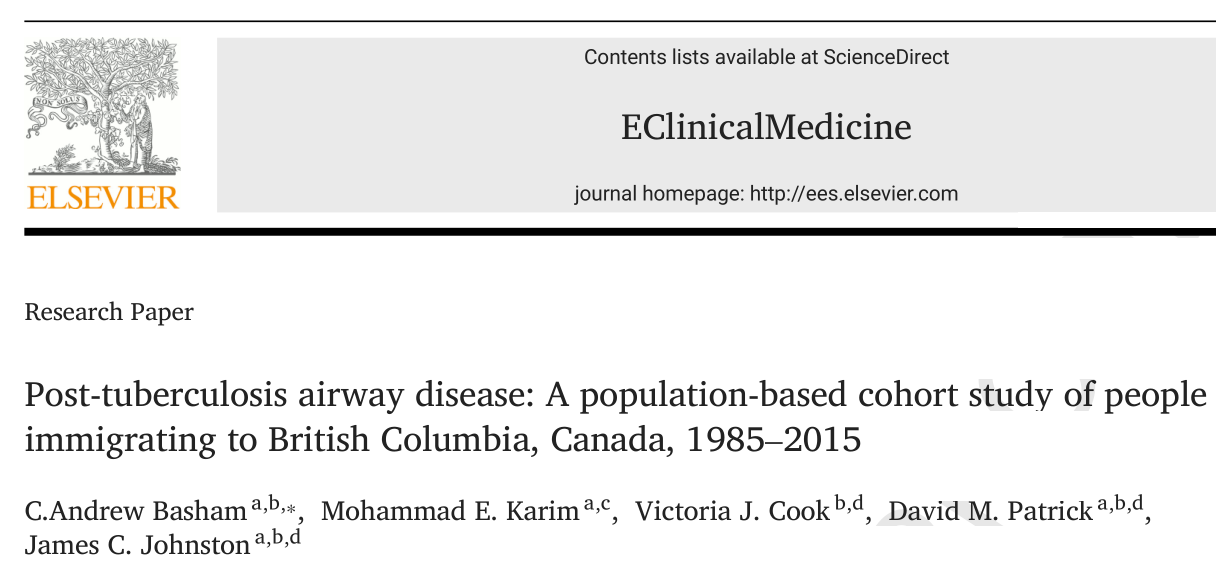
\includegraphics[width=0.5\linewidth]{paper.png}
\end{center}
\end{frame}

\begin{frame}{Questions}
\protect\hypertarget{questions}{}
Inferential goals

\begin{enumerate}
\tightlist
\item
  Prediction, developing risk scores (predict \(Y\))
\item
  Identifying important predictors (identify \(C_1\), \(C_2\) that are
  important to predict \(Y\))
\item
  Descriptive, exploratory (is \(A\) and \(Y\) associated?)
\item
  Evaluating a predictor of primary interest (does \(A\) cause \(Y\)?)
\end{enumerate}

\begin{center}
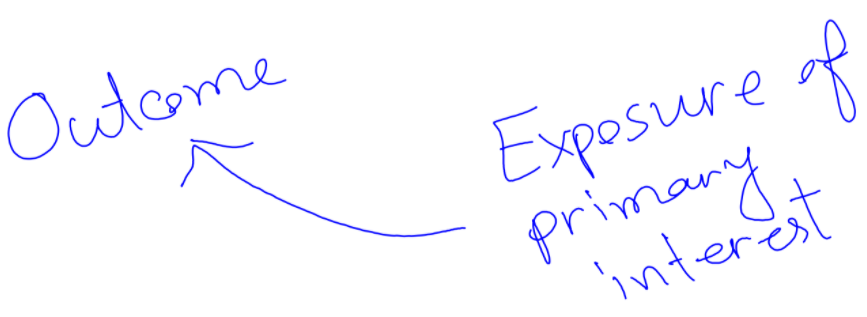
\includegraphics[width=0.7\linewidth]{p1.png} 
\end{center}

\begin{equation}
\begin{aligned}
E(Y|A,C) &= \textcolor{blue}{\psi} A \text{, after controlling for some function of C} \nonumber
\end{aligned}
\end{equation}
\end{frame}

\begin{frame}{Regression vs.~Propensity score}
\protect\hypertarget{regression-vs.-propensity-score}{}
\begin{itemize}
\tightlist
\item
  For RCT, adjustment may not be essential, as design takes care of bias
  sources.
\item
  For RWE studies, more caution necessary. Adjustment of \(C\) is
  important (\textcolor{blue}{usually large $\#$s}).
\end{itemize}

\begin{center}
\begin{tabular}{ c c c }
 \toprule
 Model / Method & Propensity score & Regression analysis \\ 
 \midrule
 Exposure Modelling & PS $ = P(A=1|C) = f(C)$ & No design stage analysis \\  
 & 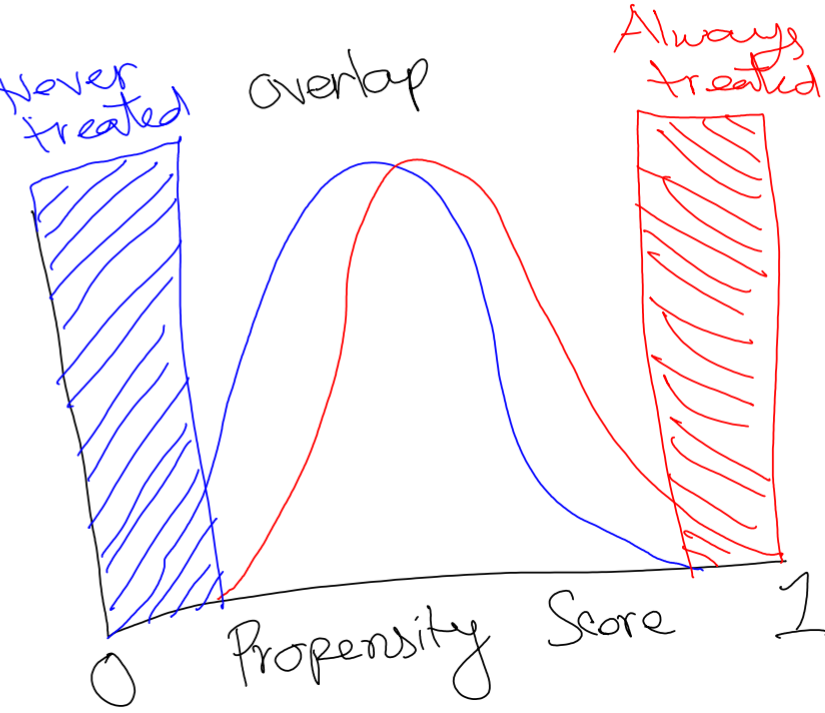
\includegraphics[width=0.25\linewidth]{overlap.png}  &  
\includegraphics[width=0.25\linewidth]{cross.png} \\
 Outcome Modelling & $E(Y|A,C) = g(A,C)$ & $E(Y|A,C) = g(A,C)$ \\    
 & in PS matched or weighted data & in full data \\    
 \bottomrule
\end{tabular}
\end{center}
\end{frame}

\begin{frame}{Health care databases}
\protect\hypertarget{health-care-databases}{}
Why use non-randomized data at all?

\begin{itemize}
\tightlist
\item
  clinical health records

  \begin{itemize}
  \tightlist
  \item
    medical facility
  \item
    hospital
  \item
    clinic and practice.
  \end{itemize}
\item
  administrative data

  \begin{itemize}
  \tightlist
  \item
    PharmaNet
  \item
    Medical Services Plan
  \end{itemize}
\item
  clinical registries

  \begin{itemize}
  \tightlist
  \item
    TB registry
  \item
    MS registry
  \end{itemize}
\end{itemize}
\end{frame}

\begin{frame}{Health care databases: Advantages}
\protect\hypertarget{health-care-databases-advantages}{}
\begin{itemize}
\tightlist
\item
  larger sample size
\item
  diverse population
\item
  longitudinal records over many years
\item
  detailed

  \begin{itemize}
  \tightlist
  \item
    health encounters,
  \item
    comorbidity history,
  \item
    drug exposure history
  \end{itemize}
\item
  possibility to link other databases

  \begin{itemize}
  \tightlist
  \item
    Immigration
  \item
    Vital Statistics
  \end{itemize}
\end{itemize}
\end{frame}

\begin{frame}{Health care databases: Study implementation}
\protect\hypertarget{health-care-databases-study-implementation}{}
Schneeweiss (2018): freeze a data cut from dynamic data stream,
encounters collected at covariate assessment period and follow-up, apply
rules/algorithms to define variables.

\begin{center}
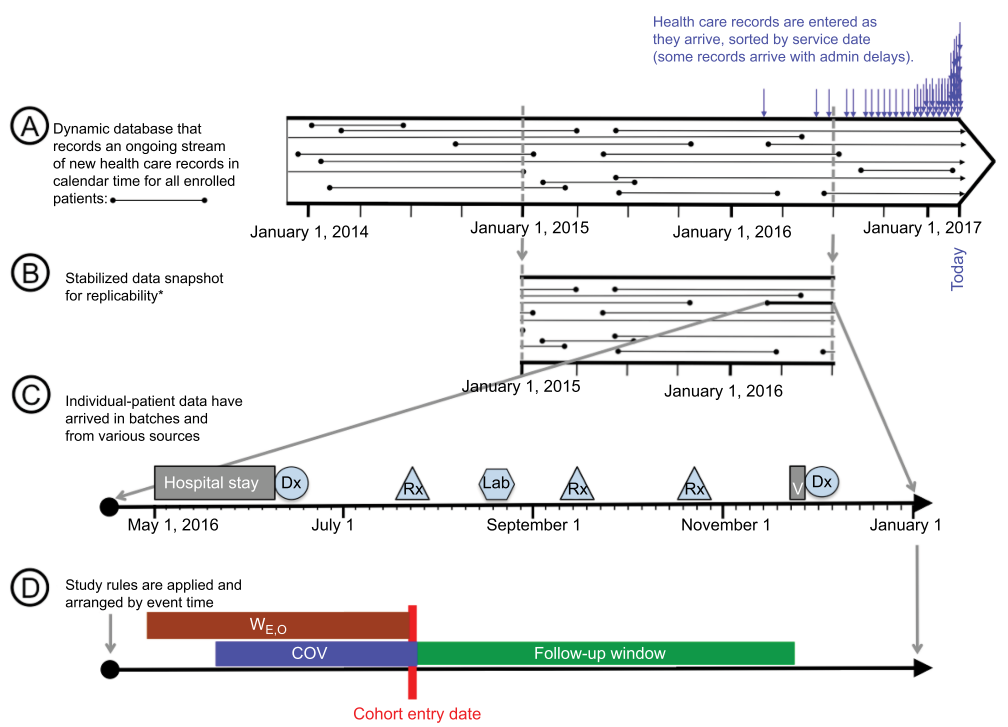
\includegraphics[width=.5\linewidth]{implementation.png}
\end{center}
\end{frame}

\begin{frame}{Health care databases: Limitations}
\protect\hypertarget{health-care-databases-limitations}{}
\begin{itemize}
\tightlist
\item
  Not specifically designed for answering a particular research question.
\item
  Data sparsity:

  \begin{itemize}
  \tightlist
  \item
    no defined or routine interview dates
  \item
    data collection relies on visits and encounters
  \end{itemize}
\item
  Investigators have no control over which factors were measured during
  the data collection stage.

  \begin{itemize}
  \tightlist
  \item
    smoking in TB
  \item
    MRI data in MS
  \end{itemize}
\end{itemize}
\end{frame}

\begin{frame}{Health care databases: Limitations}
\protect\hypertarget{health-care-databases-limitations-1}{}
\begin{center}
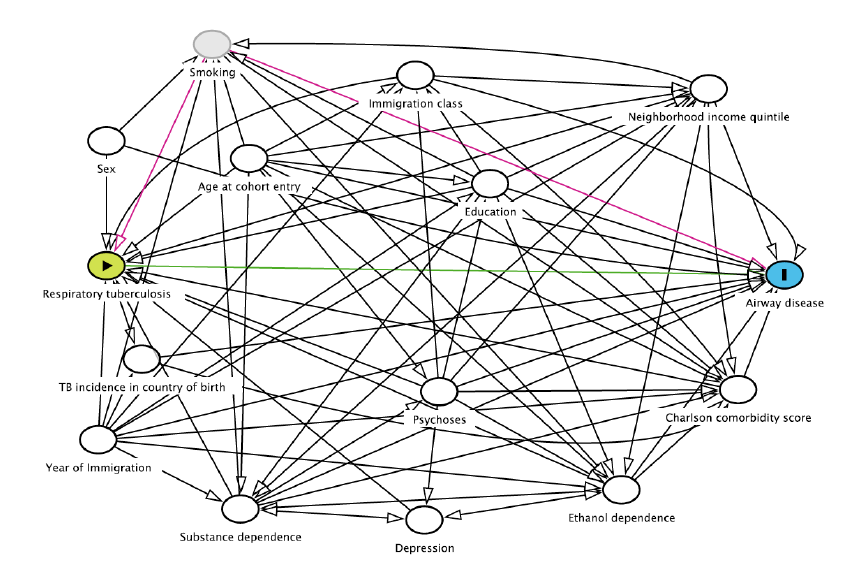
\includegraphics[width=0.65\linewidth]{dag.png}
\end{center}
\end{frame}

\begin{frame}{Methods: Expectation vs.~Reality (Part I: unmeasured
confounder)}
\protect\hypertarget{methods-expectation-vs.-reality-part-i-unmeasured-confounder}{}
\begin{block}{Exposure Model}
\protect\hypertarget{exposure-model}{}
\begin{equation}
\begin{aligned}
P(A=1|C) &= f(C) \\
        &= \frac{1}{1+exp[\alpha_0 + \alpha_1 C_1 + \alpha_2 C_2 + \alpha_3 C_3 + \alpha_4 C_4 + \alpha_5 C_5 + \alpha_6 C_6 + \alpha_7 \textcolor{blue}{C_7} ]}\nonumber
\end{aligned}
\end{equation}
\end{block}

\begin{block}{Outcome Model}
\protect\hypertarget{outcome-model}{}
\begin{equation}
\begin{aligned}
E(Y|A,C) &= g(A,C)\\
&= \beta_0 + \psi A + \beta_1 C_1 + \beta_2 C_2 + \beta_3 C_3 + \beta_4 C_4 + \beta_5 C_5 + \beta_6 C_6 + \beta_7 \textcolor{blue}{C_7} \nonumber
\end{aligned}
\end{equation}
\end{block}

\begin{block}{Assumption}
\protect\hypertarget{assumption}{}
\begin{equation} \label{eq:out2}
\begin{aligned}
Y | A,C \sim N[E(Y|A,C), \sigma^2] \nonumber
\end{aligned}
\end{equation}
\end{block}
\end{frame}

\begin{frame}{Methods: Expectation vs.~Reality (Part 2: model
misspecification)}
\protect\hypertarget{methods-expectation-vs.-reality-part-2-model-misspecification}{}
\begin{block}{Exposure Model}
\protect\hypertarget{exposure-model-1}{}
\begin{equation} 
\begin{aligned}
P(A=1|C) &= f(C) \\
        &= \frac{1}{1+exp[\alpha_0 + \alpha_1 \textcolor{blue}{(C_2 \times C_3)} + \alpha_2 \textcolor{blue}{(C_4^2 \times \frac{\exp_{C_5}}{5 \times C_7})} + \alpha_3 C_6 ]} \nonumber
\end{aligned}
\end{equation}
\end{block}

\begin{block}{Outcome Model}
\protect\hypertarget{outcome-model-1}{}
\begin{equation} 
\begin{aligned}
E(Y|A,C) &= g(A,C)\\
&= \beta_0 + \psi A + \beta_1 \textcolor{blue}{C_1^2} + \beta_2 \textcolor{blue}{(C_2 \times C_3 \times C_7)} + \beta_3 \textcolor{blue}{\frac{\exp{C_4}}{C_5 \times 2}}\nonumber
\end{aligned}
\end{equation}
\end{block}

\begin{block}{Assumption}
\protect\hypertarget{assumption-1}{}
\begin{equation} 
\begin{aligned}
Y | A,C \sim N[E(Y|A,C), \sigma^2]\nonumber
\end{aligned}
\end{equation}
\end{block}
\end{frame}

\begin{frame}[fragile]{hdPS}
\protect\hypertarget{hdps}{}
\begin{verbatim}
## Warning: package 'scholar' was built under R version 4.1.3
\end{verbatim}

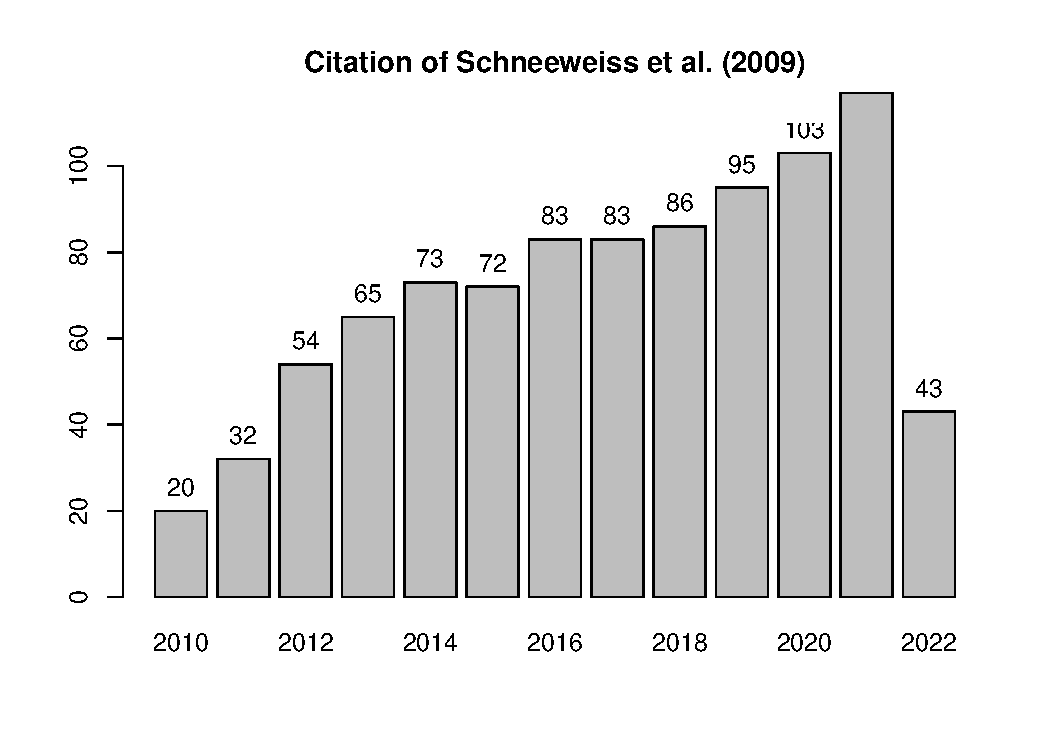
\includegraphics{slideCHSPR_files/figure-beamer/cite-1.pdf}
\end{frame}

\begin{frame}{hdPS proxy collection}
\protect\hypertarget{hdps-proxy-collection}{}
Schneeweiss (2018):

\begin{center}
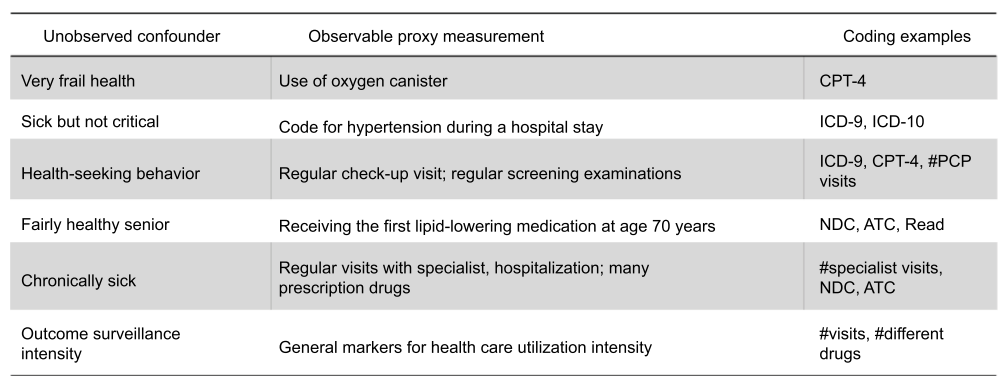
\includegraphics[width=0.5\linewidth]{code.png}
\end{center}

They were the first to propose adjusting for something that \textbf{may
not be interpretable} directly with the context of the research
question. Logic was two fold:

\begin{enumerate}
\tightlist
\item
  variables from same subject should be \textbf{correlated} = has
  relevant information
\item
  adjust items that are \textbf{predictive of outcome} (as established
  in PS literature)
\end{enumerate}
\end{frame}

\begin{frame}{hdPS proxy collection from same subjects (1)}
\protect\hypertarget{hdps-proxy-collection-from-same-subjects-1}{}
Collection of proxy data for the unmeasured + mis-measured variables
(Karim, Pang, and Platt 2018)

\begin{center}
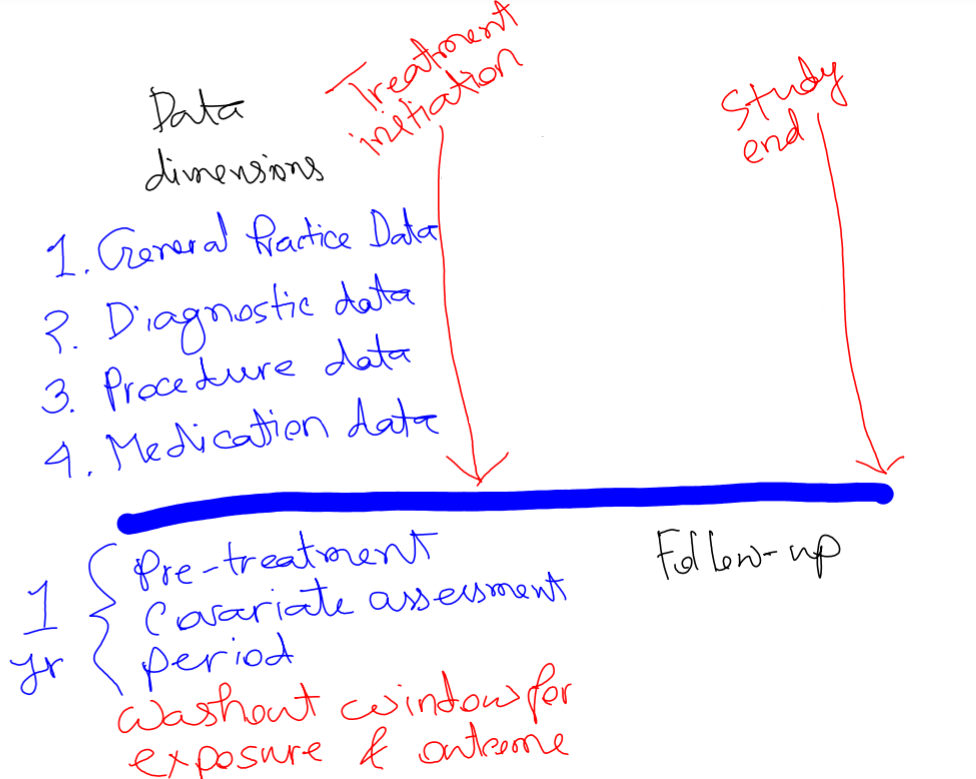
\includegraphics[width=0.45\linewidth]{proxy1.png}
\end{center}
\end{frame}

\begin{frame}{hdPS proxy collection from same subjects (1)}
\protect\hypertarget{hdps-proxy-collection-from-same-subjects-1-1}{}
Collection of proxy data for the unmeasured + mis-measured variables
(Karim, Pang, and Platt 2018)

\begin{center}
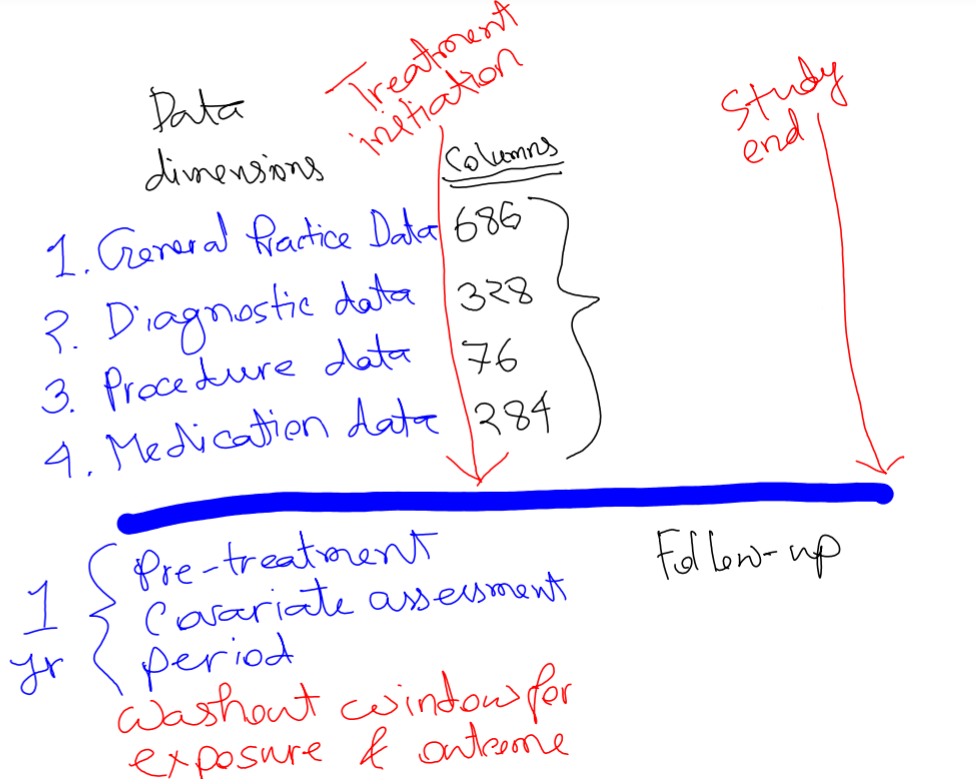
\includegraphics[width=0.45\linewidth]{proxy2.png}
\end{center}
\end{frame}

\begin{frame}{hdPS proxy collection from same subjects (1)}
\protect\hypertarget{hdps-proxy-collection-from-same-subjects-1-2}{}
Collection of proxy data for the unmeasured + mis-measured variables
(Karim, Pang, and Platt 2018)

\begin{center}
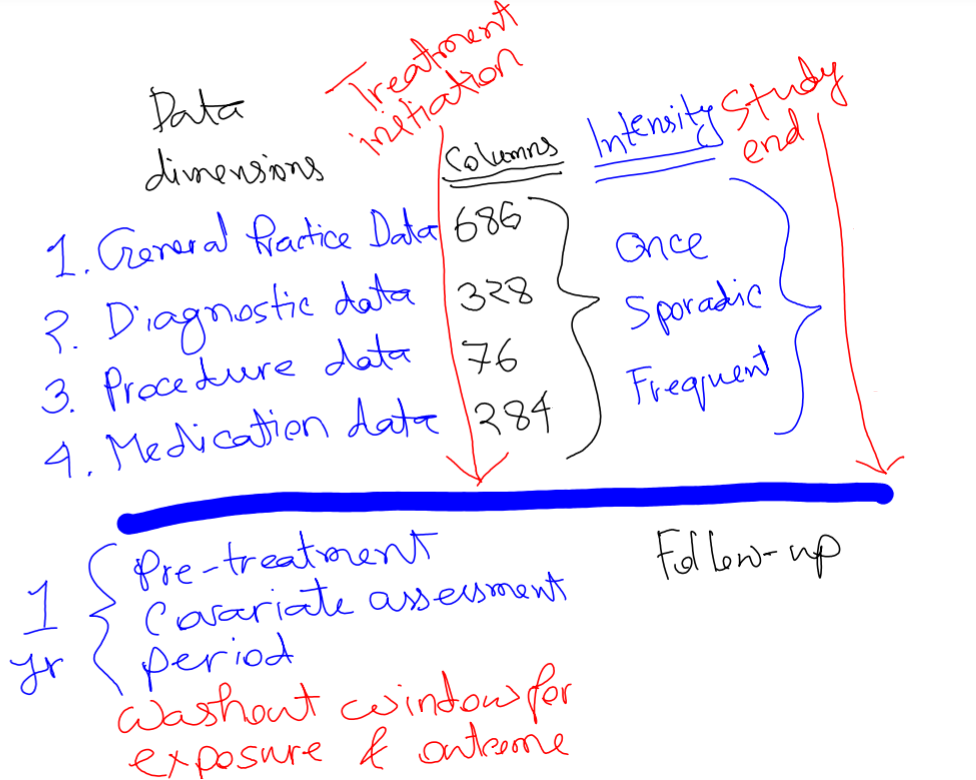
\includegraphics[width=0.45\linewidth]{proxy3.png}
\end{center}
\end{frame}

\begin{frame}{hdPS proxy collection from same subjects (1)}
\protect\hypertarget{hdps-proxy-collection-from-same-subjects-1-3}{}
Collection of proxy data for the unmeasured + mis-measured variables
(Karim, Pang, and Platt 2018): but restricted to 2,400 empirical
covariates \textcolor{blue}{EC} (based on high prevalence)

\begin{center}
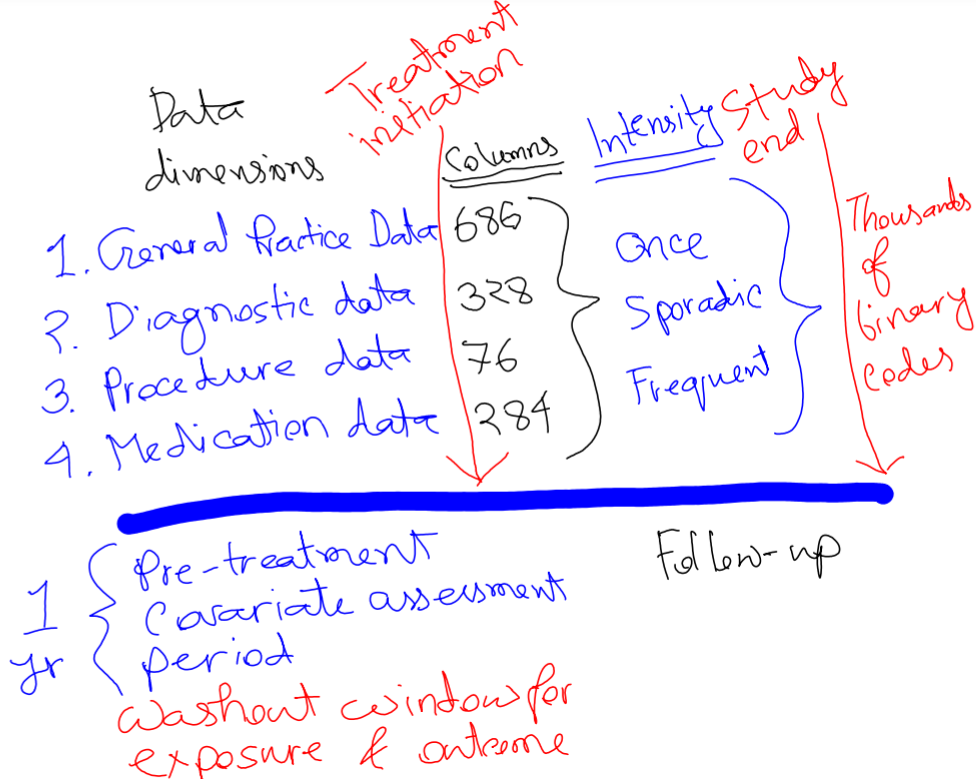
\includegraphics[width=0.45\linewidth]{proxy22.png}
\end{center}
\end{frame}

\begin{frame}{hdPS proxy collection from same subjects (1)}
\protect\hypertarget{hdps-proxy-collection-from-same-subjects-1-4}{}
List of additional proxy variables:

\begin{center}
\begin{tabular}{ c c c c }
 \toprule
Dimension 1 & Dimension 2 & Dimension 3 & Dimension 4\\
Practice  & Diagnostic & Procedure & Medication\\
 \midrule
EC-dim1-1-once & EC-dim2-1-once & EC-dim3-1-once & EC-dim4-1-once\\
EC-dim1-1-sporadic & EC-dim2-1-sporadic & EC-dim3-1-sporadic & EC-dim4-1-sporadic\\
EC-dim1-1-frequent & EC-dim2-1-frequent & EC-dim3-1-frequent & EC-dim4-1-frequent\\
$\ldots$ &  $\ldots$ & $\ldots$ \\
EC-dim1-686-frequent & EC-dim2-328-frequent & EC-dim3-76-frequent & EC-dim4-284-frequent\\
 \bottomrule
\end{tabular}
\end{center}

4 dimension \(\times\) 3 intensity \(\times\) 200 most prevalent codes =
2,400 \textcolor{blue}{EC}s
\end{frame}

\begin{frame}{hdPS mechanism: find EC as h(outcome, exposure prevalence)
(2)}
\protect\hypertarget{hdps-mechanism-find-ec-as-houtcome-exposure-prevalence-2}{}
Assumption:

\begin{itemize}
\tightlist
\item
  \(p_{u=1,a=1}\) = prevalence of unmeasured confounder among treated
  (\(A=1\))
\item
  \(p_{u=1,a=0}\) = prevalence of unmeasured confounder among untreated
  (\(A=0\))
\item
  \(p_{u=1,y=1}\) = prevalence of unmeasured confounder among dead
  (\(Y=1\))
\item
  \(p_{u=1,y=0}\) = prevalence of unmeasured confounder among alive
  (\(Y=0\))
\end{itemize}

Bross (1966) formula says, the amount of bias due to \(u\) is

\begin{equation} 
\begin{aligned}
\text{Bias}_M =  \frac{ p_{u=1,a=1} \times \Big(\frac{p_{u=1,y=1}}{p_{u=1,y=0}} -1 \Big) +1  } { p_{u=1,a=0} \times  \Big(\frac{p_{u=1,y=1}}{p_{u=1,y=0}} -1 \Big) +1}   \nonumber
\end{aligned}
\end{equation}
\end{frame}

\begin{frame}{hdPS mechanism: find EC as h(outcome, exposure prevalence)
(2)}
\protect\hypertarget{hdps-mechanism-find-ec-as-houtcome-exposure-prevalence-2-1}{}
\st{Assumption} Calculate:

\begin{itemize}
\tightlist
\item
  \(p_{\textcolor{blue}{EC}=1,a=1}\) = prevalence of
  \st{unmeasured confounder} \textcolor{blue}{EC} among treated
  (\(A=1\))
\item
  \(p_{\textcolor{blue}{EC}=1,a=0}\) = prevalence of
  \st{unmeasured confounder} \textcolor{blue}{EC} among untreated
  (\(A=0\))
\item
  \(p_{\textcolor{blue}{EC}=1,y=1}\) = prevalence of
  \st{unmeasured confounder} \textcolor{blue}{EC} among dead (\(Y=1\))
\item
  \(p_{\textcolor{blue}{EC}=1,y=0}\) = prevalence of
  \st{unmeasured confounder} \textcolor{blue}{EC} among alive (\(Y=0\))
\end{itemize}

Bross (1966) formula says, the amount of bias due to
\textcolor{blue}{EC} is

\begin{equation} 
\begin{aligned}
\text{Bias}_M =  \frac{ p_{\textcolor{blue}{EC}=1,a=1} \times \Big(\frac{p_{\textcolor{blue}{EC}=1,y=1}}{p_{\textcolor{blue}{EC}=1,y=0}} -1 \Big) +1  } { p_{\textcolor{blue}{EC}=1,a=0} \times  \Big(\frac{p_{\textcolor{blue}{EC}=1,y=1}}{p_{\textcolor{blue}{EC}=1,y=0}} -1 \Big) +1}   \nonumber
\end{aligned}
\end{equation}
\end{frame}

\begin{frame}{hdPS: select hdPS variables from ECs}
\protect\hypertarget{hdps-select-hdps-variables-from-ecs}{}
\begin{enumerate}
\tightlist
\item
  Rank (descending) each \textcolor{blue}{EC} by the magnitude of
  log-bias: \(|\log{\text{Bias}_M}|\)
\end{enumerate}

\begin{center}
\begin{tabular}{ c c c }
 \toprule
Rank by bias & $|\log{\text{Bias}_M}|$ & \textcolor{blue}{EC} \\ 
 \midrule
1 & 0.42 & EC-dim1-21-once\\
2 & 0.32 & EC-dim2-95-once\\
3 & 0.25 & EC-dim4-289-once\\
$\ldots$ &  $\ldots$ & $\ldots$ \\
2,400 & 0.01 & EC-dim4-64-frequent\\
 \bottomrule
\end{tabular}
\end{center}

\begin{enumerate}
\setcounter{enumi}{1}
\tightlist
\item
  Take top 500 of these \textcolor{blue}{EC}s. These are hdPS variables.
\end{enumerate}
\end{frame}

\begin{frame}{hdPS: estimate treatment effect}
\protect\hypertarget{hdps-estimate-treatment-effect}{}
\begin{block}{Exposure Model (investigator-specified covariates)}
\protect\hypertarget{exposure-model-investigator-specified-covariates}{}
\begin{equation}
\begin{aligned}
P(A=1|C) &= f(C) \\
        &= \frac{1}{1+exp[\alpha_0 + \alpha_1 C_1 + \alpha_2 C_2 + \alpha_3 C_3 + \alpha_4 C_4 + \alpha_5 C_5 + \alpha_6 C_6 + \alpha_7 \textcolor{blue}{C_7} ]}\nonumber
\end{aligned}
\end{equation}
\end{block}

\begin{block}{Outcome Model (in the PS matched or weighted data)}
\protect\hypertarget{outcome-model-in-the-ps-matched-or-weighted-data}{}
\begin{equation}
\begin{aligned}
E(Y|A,C) &= g(A,C)\\
&= \beta_0 + \psi A \nonumber
\end{aligned}
\end{equation}
\end{block}
\end{frame}

\begin{frame}{hdPS: estimate treatment effect}
\protect\hypertarget{hdps-estimate-treatment-effect-1}{}
\begin{block}{Exposure Model (investigator-specified covariates + hdPS
variables {[}EC{]})}
\protect\hypertarget{exposure-model-investigator-specified-covariates-hdps-variables-ec}{}
\begin{equation}
\begin{aligned}
P(A=1|C) &= f(C) \\
        &= \frac{1}{1+exp[\alpha_0 + \alpha_1 C_1 + \alpha_2 C_2 + \alpha_3 C_3 + \alpha_4 C_4 + \alpha_5 C_5 + \alpha_6 C_6 +  \sum_{i=1}^{500} \alpha_i^{'} \textcolor{blue}{\text{EC}_i} ]}\nonumber
\end{aligned}
\end{equation}
\end{block}

\begin{block}{Outcome Model (in the PS matched or weighted data)}
\protect\hypertarget{outcome-model-in-the-ps-matched-or-weighted-data-1}{}
\begin{equation}
\begin{aligned}
E(Y|A,C) &= g(A,C)\\
&= \beta_0 + \psi A \nonumber
\end{aligned}
\end{equation}
\end{block}
\end{frame}

\begin{frame}{hdPS: estimate treatment effect}
\protect\hypertarget{hdps-estimate-treatment-effect-2}{}
Performance of hdPS. Schneeweiss (2018):

\begin{center}
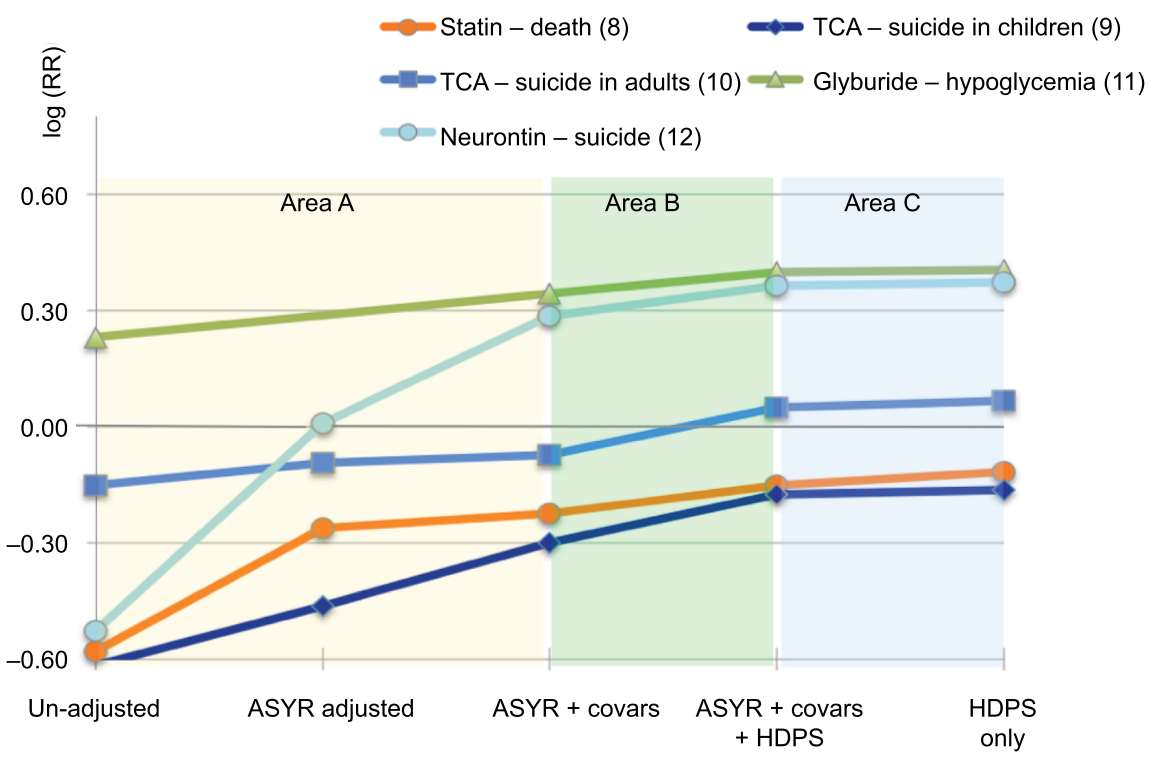
\includegraphics[width=0.6\linewidth]{hdpsonly.png}
\end{center}
\end{frame}

\begin{frame}{ML-hdPS: deal with collinearity}
\protect\hypertarget{ml-hdps-deal-with-collinearity}{}
\begin{block}{Kitchen SSink Exposure Model (A \textasciitilde{} C + EC)}
\protect\hypertarget{kitchen-ssink-exposure-model-a-c-ec}{}
\begin{equation}
\begin{aligned}
P(A=1|C, EC) &= \frac{1}{1+exp[\alpha_0 + \alpha_1 C_{\text{important}} + \alpha_2 C_{\text{potential confounder}} +  \sum_{i=1}^{2,400} \alpha_i^{'} \textcolor{blue}{\text{EC}_i} ]}\nonumber
\end{aligned}
\end{equation}
\end{block}

\begin{block}{Outcome Model for EC selection (Y \textasciitilde{} C +
top-500 ECs)}
\protect\hypertarget{outcome-model-for-ec-selection-y-c-top-500-ecs}{}
\begin{equation}
\begin{aligned}
f(Y|C, EC) &= \alpha_0 + \alpha_1 C_{\text{important}} + \alpha_2 C_{\text{potential confounder}} +  \sum_{i=1}^{500} \alpha_i^{'} \textcolor{blue}{\text{EC}_i} \nonumber
\end{aligned}
\end{equation}
\end{block}
\end{frame}

\begin{frame}{ML-hdPS: deal with collinearity}
\protect\hypertarget{ml-hdps-deal-with-collinearity-1}{}
\begin{block}{hdPS Exposure Model (A \textasciitilde{} C + top-ranked
EC)}
\protect\hypertarget{hdps-exposure-model-a-c-top-ranked-ec}{}
\begin{equation}
\begin{aligned}
P(A=1|C, EC) &= \frac{1}{1+exp[\alpha_0 + \alpha_1 C_{\text{important}} + \alpha_2 C_{\text{potential confounder}} +  \sum_{i=1}^{\text{top 500}} \alpha_i^{'} \textcolor{blue}{\text{EC}_i} ]}\nonumber
\end{aligned}
\end{equation}
\end{block}

\begin{block}{Outcome Model for EC selection (Y \textasciitilde{} C +
ECs)}
\protect\hypertarget{outcome-model-for-ec-selection-y-c-ecs}{}
\begin{equation}
\begin{aligned}
f(Y|C, EC) &= {\alpha_0 + \alpha_1 C_{\text{important}} + \alpha_2 C_{\text{potential confounder}} +  \sum_{i=1}^{2,400} \alpha_i^{'} \textcolor{blue}{\text{EC}_i} }\nonumber
\end{aligned}
\end{equation}
\end{block}
\end{frame}

\begin{frame}{ML-hdPS: deal with collinearity}
\protect\hypertarget{ml-hdps-deal-with-collinearity-2}{}
\begin{block}{Exposure Model (investigator-specified covariates + hdPS
variables {[}EC{]})}
\protect\hypertarget{exposure-model-investigator-specified-covariates-hdps-variables-ec-1}{}
\begin{equation}
\begin{aligned}
P(A=1|C) &= \frac{1}{1+exp[\alpha_0 + \alpha_1 C_1 + \alpha_2 C_2 + \alpha_3 C_3 + \alpha_4 C_4 + \alpha_5 C_5 + \alpha_6 C_6 +  \sum_{i=1}^{500} \alpha_i^{'} \textcolor{blue}{\text{EC}_i} ]}\nonumber
\end{aligned}
\end{equation}
\end{block}

\begin{block}{ML extensions: exposure model vs.~outcome model}
\protect\hypertarget{ml-extensions-exposure-model-vs.-outcome-model}{}
\begin{itemize}
\tightlist
\item
  \textcolor{blue}{\text{EC}}s selected separately

  \begin{itemize}
  \tightlist
  \item
    are usually highly correlated, and
  \item
    has inflated variance.
  \end{itemize}
\item
  Karim, Pang, and Platt (2018) used elasic net and LASSO to reduce the
  number of selected hdPS variables (\textcolor{blue}{\text{EC}}
  variables).

  \begin{itemize}
  \tightlist
  \item
    found that the hybrid method (elastic net of hdPS) performs better
    than ML or hdPS.
  \item
    quality of proxy information matters.
  \end{itemize}
\end{itemize}
\end{block}
\end{frame}

\begin{frame}{ML-hdPS: deal with model misspecification}
\protect\hypertarget{ml-hdps-deal-with-model-misspecification}{}
\begin{block}{Exposure Model}
\protect\hypertarget{exposure-model-2}{}
\begin{equation} 
\begin{aligned}
P(A=1|C) &= \frac{1}{1+exp[\alpha_0 + \alpha_1 \textcolor{blue}{(C_2 \times C_3)} + \alpha_2 \textcolor{blue}{(C_4^2 \times \frac{\exp_{C_5}}{5 \times C_7})} + \alpha_3 C_6 ]} \nonumber
\end{aligned}
\end{equation}
\end{block}

\begin{block}{Outcome Model}
\protect\hypertarget{outcome-model-2}{}
\begin{equation} 
\begin{aligned}
E(Y|A,C) &= \beta_0 + \psi A + \beta_1 \textcolor{blue}{C_1^2} + \beta_2 \textcolor{blue}{(C_2 \times C_3 \times C_7)} + \beta_3 \textcolor{blue}{\frac{\exp{C_4}}{C_5 \times 2}}\nonumber
\end{aligned}
\end{equation}
\end{block}

\begin{block}{More ML extensions}
\protect\hypertarget{more-ml-extensions}{}
\begin{itemize}
\tightlist
\item
  Tree-based models: automatically detect function form

  \begin{itemize}
  \tightlist
  \item
    Karim, Pang, and Platt (2018) used random forest, and chose top
    important \textcolor{blue}{\text{EC}}s
  \end{itemize}
\item
  Superlearner (ensemble learner) with tree-based + parametric models
\item
  Double robust methods with Superlearner
\end{itemize}
\end{block}
\end{frame}

\begin{frame}{AI-hdPS: towads dimension reduction}
\protect\hypertarget{ai-hdps-towads-dimension-reduction}{}
\begin{itemize}
\tightlist
\item
  Principal component (\textcolor{blue}{PC}) analysis

  \begin{itemize}
  \tightlist
  \item
    compute linear transformation of all covariates to
    \textcolor{blue}{PC}s, and top few \textcolor{blue}{PC}s are
    selected to reduce dimension.
  \item
    extract components of each variable resoponsible for most variance
  \item
    incapable of learning non-linear feature representations
  \end{itemize}
\end{itemize}
\end{frame}

\begin{frame}{AI-hdPS: towads dimension reduction}
\protect\hypertarget{ai-hdps-towads-dimension-reduction-1}{}
\begin{itemize}
\tightlist
\item
  Weberpals et al. (2021) proposed to use \textcolor{blue}{autoencoders}
  (3, 5, 7 layers) to reduce \textcolor{blue}{EC} dimensions:
\end{itemize}

\begin{center}
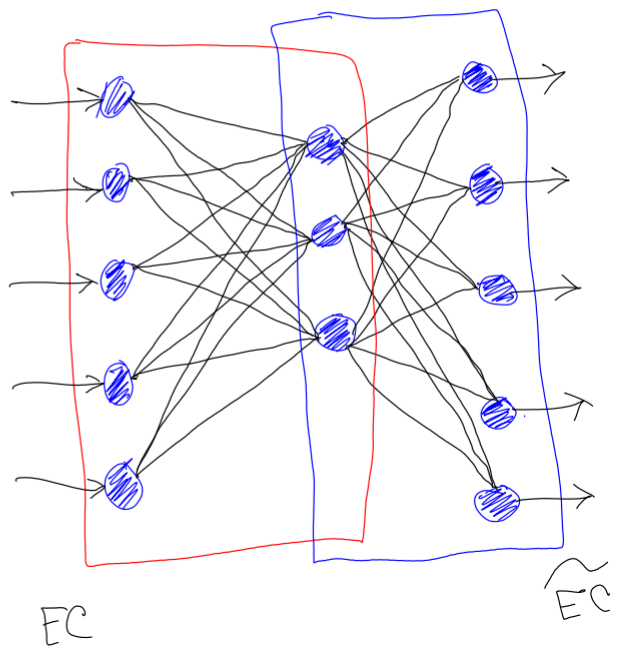
\includegraphics[width=0.3\linewidth]{ae.png}
\end{center}
\end{frame}

\begin{frame}{AI-hdPS: towads dimension reduction}
\protect\hypertarget{ai-hdps-towads-dimension-reduction-2}{}
\% Bias

\begin{center}
\includegraphics[width=0.5\linewidth]{Bias.png}
\end{center}
\end{frame}

\begin{frame}{AI-hdPS: towads dimension reduction}
\protect\hypertarget{ai-hdps-towads-dimension-reduction-3}{}
rMSE

\begin{center}
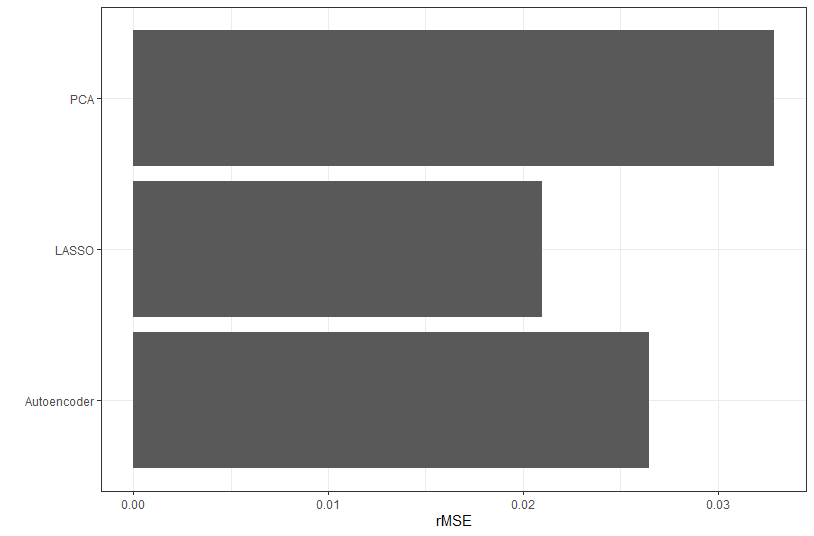
\includegraphics[width=0.5\linewidth]{rMSE.png}
\end{center}
\end{frame}

\begin{frame}{AI-hdPS: towads dimension reduction}
\protect\hypertarget{ai-hdps-towads-dimension-reduction-4}{}
Coverage: slower rate of convergence for non-parametric methods

\begin{center}
\includegraphics[width=0.5\linewidth]{Coverage.png}
\end{center}
\end{frame}

\begin{frame}{Future directions}
\protect\hypertarget{future-directions}{}
Zivich and Breskin (2021): Cross-fitting + together with double-robust
approaches

\begin{center}
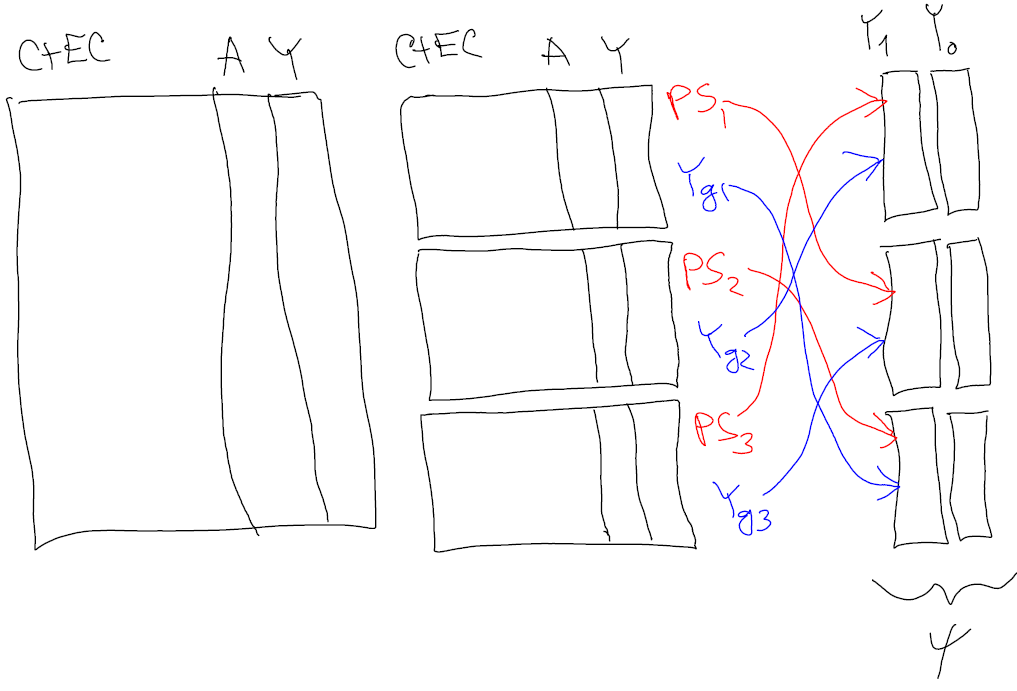
\includegraphics[width=0.6\linewidth]{cf.png} 
\end{center}
\end{frame}

\begin{frame}{A purist view}
\protect\hypertarget{a-purist-view}{}
\begin{itemize}
\tightlist
\item
  Bias-based hdPS is not really PS!

  \begin{itemize}
  \tightlist
  \item
    design stage vs.~analysis stage
  \item
    hdPS uses corr(EC, outcome).
  \end{itemize}
\item
  Motivation of PS and hdPS are different to begin with

  \begin{itemize}
  \tightlist
  \item
    PS requires no unmeasured confounding
  \end{itemize}
\item
  I prefer to use hdPS as a sensitivity analysis.
\end{itemize}
\end{frame}

\begin{frame}{Examples of hdPS (1)}
\protect\hypertarget{examples-of-hdps-1}{}
\begin{center}
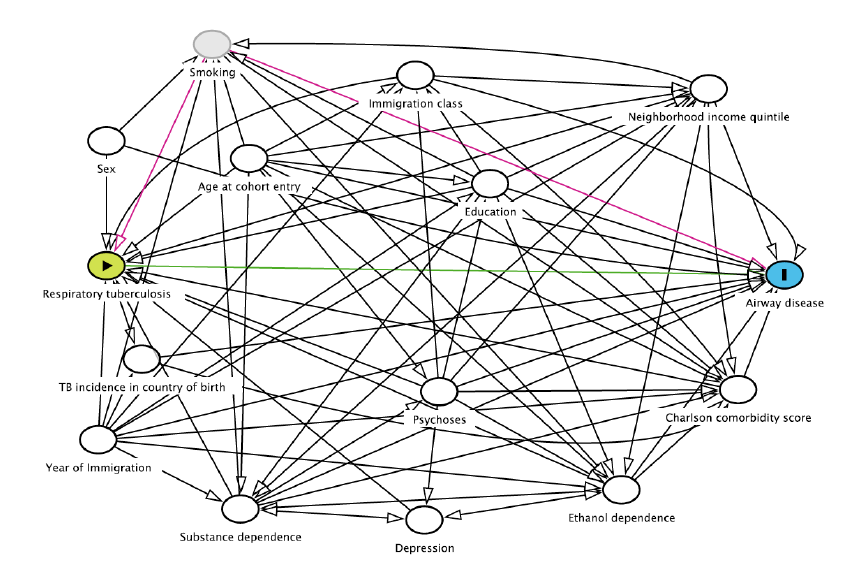
\includegraphics[width=0.3\linewidth]{dag.png}
\end{center}

Airway example: analysis approaches that were compared: hdPS as
\textcolor{blue}{sensitivity analyses}:

\begin{itemize}
\tightlist
\item
  PS decile-adjusted (investigator-specified covariates)
\item
  hdPS decile-adjusted (investigator-specified +
  \textcolor{blue}{\text{EC}})
\item
  LASSO-hdPS decile-adjusted (investigator-specified + LASSO-reduce
  \textcolor{blue}{\text{EC}})
\item
  Others: E-value, other proxy variable adjustment
\end{itemize}

Conclusions were similar.
\end{frame}

\begin{frame}{Examples of hdPS (2)}
\protect\hypertarget{examples-of-hdps-2}{}
A 2017 JAMA paper

\begin{center}
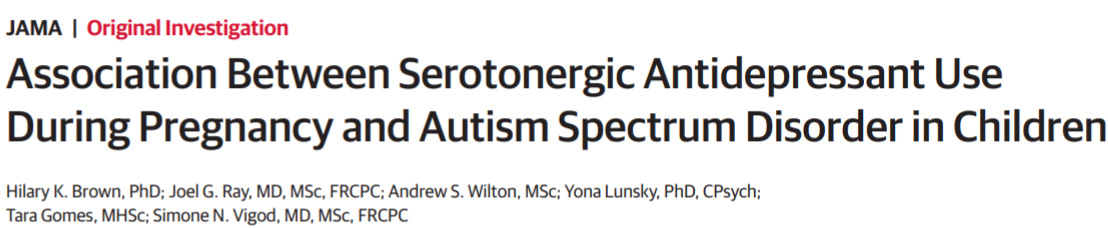
\includegraphics[width=0.5\linewidth]{jama.png} 
\end{center}

\begin{center}
\begin{tabular}{ c c c }
 \toprule
Method & HR & CI $95\%$ \\ 
 \midrule
Unadjusted & 2.16 & 1.64-2.86\\
Multivariable adjusted & 1.59 & 1.17-2.17\\
IPTW hdPS & \textcolor{blue}{1.61} & \textcolor{blue}{0.997-2.59}\\
1-1 hdPS matching &  1.64 & 1.07-2.53\\
Pre-pregnancy data & 1.85 & 1.37-2.51\\
 \bottomrule
\end{tabular}
\end{center}

Conclusion: \textbf{not associated}!
\end{frame}

\begin{frame}{Reference}
\protect\hypertarget{reference}{}
\hypertarget{refs}{}
\begin{CSLReferences}{1}{0}
\leavevmode\vadjust pre{\hypertarget{ref-karim2018can}{}}%
Karim, Mohammad Ehsanul, Menglan Pang, and Robert W Platt. 2018. {``Can
We Train Machine Learning Methods to Outperform the High-Dimensional
Propensity Score Algorithm?''} \emph{Epidemiology} 29 (2): 191--98.

\leavevmode\vadjust pre{\hypertarget{ref-schneeweiss2018automated}{}}%
Schneeweiss, Sebastian. 2018. {``Automated Data-Adaptive Analytics for
Electronic Healthcare Data to Study Causal Treatment Effects.''}
\emph{Clinical Epidemiology} 10: 771--78.

\leavevmode\vadjust pre{\hypertarget{ref-weberpals2021deep}{}}%
Weberpals, Janick, Tim Becker, Jessica Davies, Fabian Schmich, Dominik
Rüttinger, Fabian J Theis, and Anna Bauer-Mehren. 2021. {``Deep
Learning-Based Propensity Scores for Confounding Control in Comparative
Effectiveness Research: A Large-Scale, Real-World Data Study.''}
\emph{Epidemiology, Doi: 10.1097/EDE.0000000000001338}.

\leavevmode\vadjust pre{\hypertarget{ref-zivich2020machine}{}}%
Zivich, Paul N, and Alexander Breskin. 2021. {``Machine Learning for
Causal Inference: On the Use of Cross-Fit Estimators.''}
\emph{Epidemiology, Doi: 10.1097/EDE.0000000000001332}.

\end{CSLReferences}
\end{frame}

\begin{frame}{Thank you!}
\protect\hypertarget{thank-you}{}
\begin{center}

\includegraphics[width=1\linewidth]{site.png} 
\end{center}
\end{frame}

\end{document}
